\chapter{Introduction}

This chapter is an introduction to the topic of the thesis. It gives the reader an idea of the problem at hand and why it is relevant. Simplified pictures and illustrations help to understand the problem on a general level. 

\section{Packages}
This template already comes with a large variety of packages. \textsc{Before you add custom packages please check if they are not already included in} \texttt{ACSDthesis\_config.tex}\textsc{, since double inclusions can interfere with options and destroy the layout!} Table \ref{tab:packages} lists all included packages with their according options. If you need to add custom options for a specific package, use the \texttt{\textbackslash PassOptionsToPackage\{<options>\}\{<package>\}} command, \textsc{before} the package is included.
\begin{table}[H]
\centering
\caption{Packages included in this template. The entry \textit{cf. config} refers to the file \texttt{ACSDthesis\_config.tex}, where extended setups are included.}
\begin{tabular}{l | l || l | l || l | l}
Package			& Options 			& Package			& Options 			& Package			& Options 			\\ \hline
accents				&					&
acronym			& smaller			&
algorithm2e		&\textit{cf. config}	\\
amsmath			&					&
amsthm			&					&
amssymb			&					\\
amsfonts			&					&
babel				& ngerman	/english&
calc				&					\\
caption				&\textit{cf. config}	&
csquotes			&\textit{cf. config}	&
epsfig				&					\\
epstopdf			&					&
enumerate			&					&
fontenc				& T1				\\
fixltx2e				&					&
graphicx			& pdftex			&
here				&					\\
listings				&\textit{cf. config}	&
mparhack			&					&
multicol			&					\\
pdfpages			&					&
pstricks				&					&
scrhack				&					\\
subcaption			&					&
textcomp			&					&
tikz					&					\\
units				&					&
xcolor				& dvipsnames		&
xspace				&				
\end{tabular}
\label{tab:packages}
\end{table}

\section{Citation}
At some point in your thesis you will have to cite another author's work. If not you either did something extremely wrong or extremely right.\footnote{But probably the first of the two.} This template uses the \texttt{csquotes} package for citation, which is set up in the file \texttt{ACSDthesis\_config.tex}. In order to cite use the \texttt{\textbackslash cite\{<bibtexkey>\}} command. Natbib citation commands like \texttt{\textbackslash citet\{\}} are also supported. Table \ref{tab:citation} shows the different available commands and their results.

If you cite more than one paper at a time, \textsc{put them all in a comma-separated list within the same cite command!} For example, \texttt{\textbackslash cite\{Betti2013, Picasso2016\}} produces \cite{Betti2013, Picasso2016} and \texttt{\textbackslash cite\{Limon2008, Betti2013, Picasso2016\}} produces \cite{Limon2008, Betti2013, Picasso2016}.

\begin{table}[H]
\centering
\caption{Citation styles supported in this thesis using the bibtexkey \textit{Limon2008} as an example. If not otherwise specified by your supervisor, use the \texttt{\textbackslash cite\{<bibtexkey>\}} command.} 
\begin{tabular}{l | l }
Command & Result \\ \hline
\texttt{\textbackslash cite\{Limon2008\}}			& \cite{Limon2008}			\\
\texttt{\textbackslash cite[see][chap. 2]\{Limon2008\}} & \cite[see][chap. 2]{Limon2008} \\
\texttt{\textbackslash citet\{Limon2008\}}			& \citet{Limon2008}			\\
\texttt{\textbackslash citet*\{Limon2008\}}		& \citet*{Limon2008}		\\
\texttt{\textbackslash citeauthor\{Limon2008\}}	& \citeauthor{Limon2008}	\\
\texttt{\textbackslash citeyear\{Limon2008\}}		& \citeyear{Limon2008}	
\end{tabular}
\label{tab:citation}
\end{table}

\section{Block Diagrams and Code Snippets}
A small example of a simple block diagram in tikz is shown in Figure \ref{fig:simpletikz}. The according code is the following: 
\lstset{language=TeX} % HERE IS HOW TO INCLUDE SCOURCE CODE SNIPPETS IN YOUR TEXT
\begin{lstlisting}
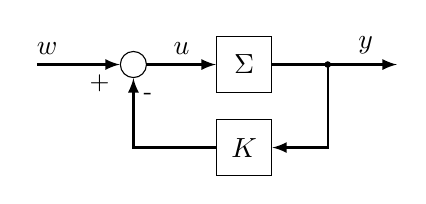
\begin{tikzpicture}
\tikzstyle{arrow} = [thick, color = black, -latex] % define standard arrow
\tikzstyle{block} = [draw, rectangle, minimum height = 2em, minimum width = 2em, align = center] % define standard block
\tikzstyle{dot} = [draw, shape = circle, inner sep = 0em, minimum size=0.15em, fill = black] % small dot on line junctions
\node(system)[block] at (0,0){$\Sigma$}; % draw system block at (0,0) -> reference for other stuff
\draw[arrow](system.east)--++(4.5em,0)node[near end, above]{$y$}; % draw output arrow of length 4em from sys block
\node(controller)[block, below of = system, node distance = 3em]{$K$}; % draw controller gain block
\draw[arrow](system.east)++(2em,0)node[dot]{}|-(controller.east); % draw arrow from output signal to controller gain
\node(sum)[draw, shape = circle, radius = 0.25em, left of = system, node distance = 4em]{}; % draw summation point
% draw arrows that connect with the summation point
\draw[arrow](controller.west)-|(sum.south)node[below right]{\small -}; % feedback
\draw[arrow](sum.west)++(-3em,0)--(sum.west)node[very near start, above]{$w$}node[below left]{\small +}; % reference
\draw[arrow](sum.east)--(system.west)node[midway, above]{$u$}; % input
\end{tikzpicture}
\end{lstlisting}

This was also an example of how to add code blocks to your text using the listings environment. The according setup is included in the file \texttt{ACSDthesis\_config.tex}. 

\begin{figure}
\centering
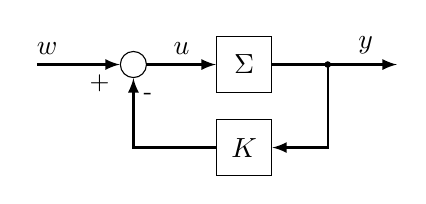
\begin{tikzpicture} % THIS IS A SIMPLE BLOCK DIAGRAM DONE IN TIKZ
\tikzstyle{arrow} 	= [thick, color = black, -latex] % define standard arrow
\tikzstyle{block} 	= [draw, rectangle, minimum height = 2em, minimum width = 2em, align=center] % define standard block
\tikzstyle{dot} 		= [draw, shape = circle, inner sep = 0em, minimum size=0.15em, fill=black] % small dot on line junctions

\node(system)[block] at (0,0){$\Sigma$}; % draw system block at (0,0) -> reference for other stuff
\draw[arrow](system.east)--++(4.5em,0)node[near end, above]{$y$}; % draw output arrow of length 4em from sys block
\node(controller)[block, below of = system, node distance = 3em]{$K$}; % draw controller gain block
\draw[arrow](system.east)++(2em,0)node[dot]{}|-(controller.east); % draw arrow from output signal to controller gain
\node(sum)[draw, shape = circle, radius = 0.25em, left of = system, node distance = 4em]{}; % draw summation point

% draw arrows that connect with the summation point
\draw[arrow](controller.west)-|(sum.south)node[below right]{\small -}; % feedback
\draw[arrow](sum.west)++(-3em,0)--(sum.west)node[very near start, above]{$w$}node[below left]{\small +}; % reference
\draw[arrow](sum.east)--(system.west)node[midway, above]{$u$}; % input
\end{tikzpicture}
\caption[Basic block diagrams in tikz]{This is an example for a simple block diagram using tikz.}
\label{fig:simpletikz}
\end{figure}

Note that it is often times a good idea to not write your tikz code directly in the source code, but to store it in a separate file and use the \texttt{\textbackslash input\{\}} command instead. This was for example done with Figure \ref{fig:problem}. 

\section{Definitions, Theorems, and so forth}
If you want to include definitions or theorems just use the respective environment, which are created with the usual \texttt{\textbackslash begin\{\}} and \texttt{\textbackslash end\{\}} commands. Available environments are \texttt{definition}, \texttt{assumption}, \texttt{lemma}, \texttt{theorem}, \texttt{proof}, and \texttt{remark}. It is of course also possible to reference them in the usual way.

\begin{definition}[Convexity]
A function $f:\mathcal{X}\to\mathcal{R}$ is called \textbf{convex}, if $\forall x, y\in\mathcal{X}, \forall t\in[0,1]:$ 
$f(tx+(1-t)y)\leq tf(x) + (1-t)f(y).$
\label{def:convexity}
\end{definition}
\begin{lemma}[Sum of convex functions]
Let $f:\mathcal{X}\to\mathcal{R}$ and $g:\mathcal{X}\to\mathcal{R}$ be two convex functions. Then the sum $h(x) = f(x)+g(x)$ is also convex.
\label{lem:sumconvex}
\end{lemma}
\begin{proof}[Proof of Lemma \ref{lem:sumconvex}]
The proof is trivial and follows directly from Definition \ref{def:convexity}. \qedhere
\end{proof}
\begin{remark}
Don't do proofs like that!
\end{remark}
